\section{Results}
\subsection{Initial Code, Importance Sampling, and Statistical Analysis}

\begin{table}
\begin{tabular}{l|c|c}
	Mean time for simulations & $5.88E-5$ s & \\
	\hline
	$\gamma$ & $\expect{E}$ a.u & Mean Variance $\sqrt{\sigma}$\\
	\hline
	$1E-3$ & $4.25093$ & $2.99E-2$ \\
	$1E-2$ & $3.26251$ & $2.99E-2$ \\
	$1E-1$ & $3.00228$ & $2.99E-2$ \\
	$4E-1$ & $3.00023$ & $2.99E-2$ \\
\end{tabular}
\label{tab:naive-nin}
\caption{Gamma comparisons for brute force metropolis sampling.}
\end{table}

\subsection{Gibbs sampling}
Figure \ref{fig:1f_1}, \ref{fig:1f_2} and \ref{fig:1f_3} show simulations for the system using Gibbs sampling. In \ref{fig:1f_1} we see the results for one particle for 1, 2 and 3 dimensions. For all cases we see that the higher $\gamma$ the faster the gradient descent method moves towards an the expectation energy, however they are not the right values. In the case of one particle in one dimension the expectation value keeps dropping to infinity. \\
For the two particle case we still have a factorization problem, the energy stabilizes at wrong energies.\\
In figure \ref{fig:1f_3} we see how the simulations evolve using different values of standard deviation $\sigma$. For small $\sigma$ we draw new values for the visible units from a smaller range in position space and for bigger $\sigma$ we draw from a broader range. Calculating new moves with a higher standard deviation could cause the method to moves faster. And we see that the slope for high $\sigma$ is steeper than for smaller $\sigma$. However the energies are again wrong.


\subsection{Interaction}
We add the simple coloumb interaction to the program and opt to use the brute force metropolis algorithm as it was the most stable over the model hyperparameters, e.g. $\gamma$. Simulatig for the $N = D = 2$ case granted results as can be seen in figure \ref{fig:inter} and table \ref{tab:inter}. We observe an instability around the reported analytic mean of 3 a.u. And also no seeming great impact of variations of the paramete $\gamma$ on the scale $1e-1$. More rigorous analysis of the significance of these changes were however not performed. 

\begin{table}
	\begin{tabular}{|L|c|c|}
	\hline
$\gamma$ & $\textit{mean}(\expect{E})$ & $\textit{mean}(\sigma ^2)$ \\
\hline \hline
$3.00e-01$ & $3.10432$ & $4.11e-02$ \\
$4.00e-01$ &  $3.10004$ & $4.07e-02$ \\
$5.00e-01$ &  $3.10643$ & $4.15e-02$ \\
\hline
	\end{tabular}
\caption{Simulating the $N = D = 2$ system with an added coloumb interaction led to a more oscillating behaviour than for the non-interactive case. This can be seen in figure \ref{fig:inter}. The simulation was run for 200 gradient descent iterations, the means were taken over the last 160 of them to capture only the oscillation and not the convergence. We observe that gamma does not seeem to have a dramatic impact on the stability in this case. The mean time for the simulations was $2.97e-04$ seconds}\label{tab:inter}
\end{table}


\begin{figure}
	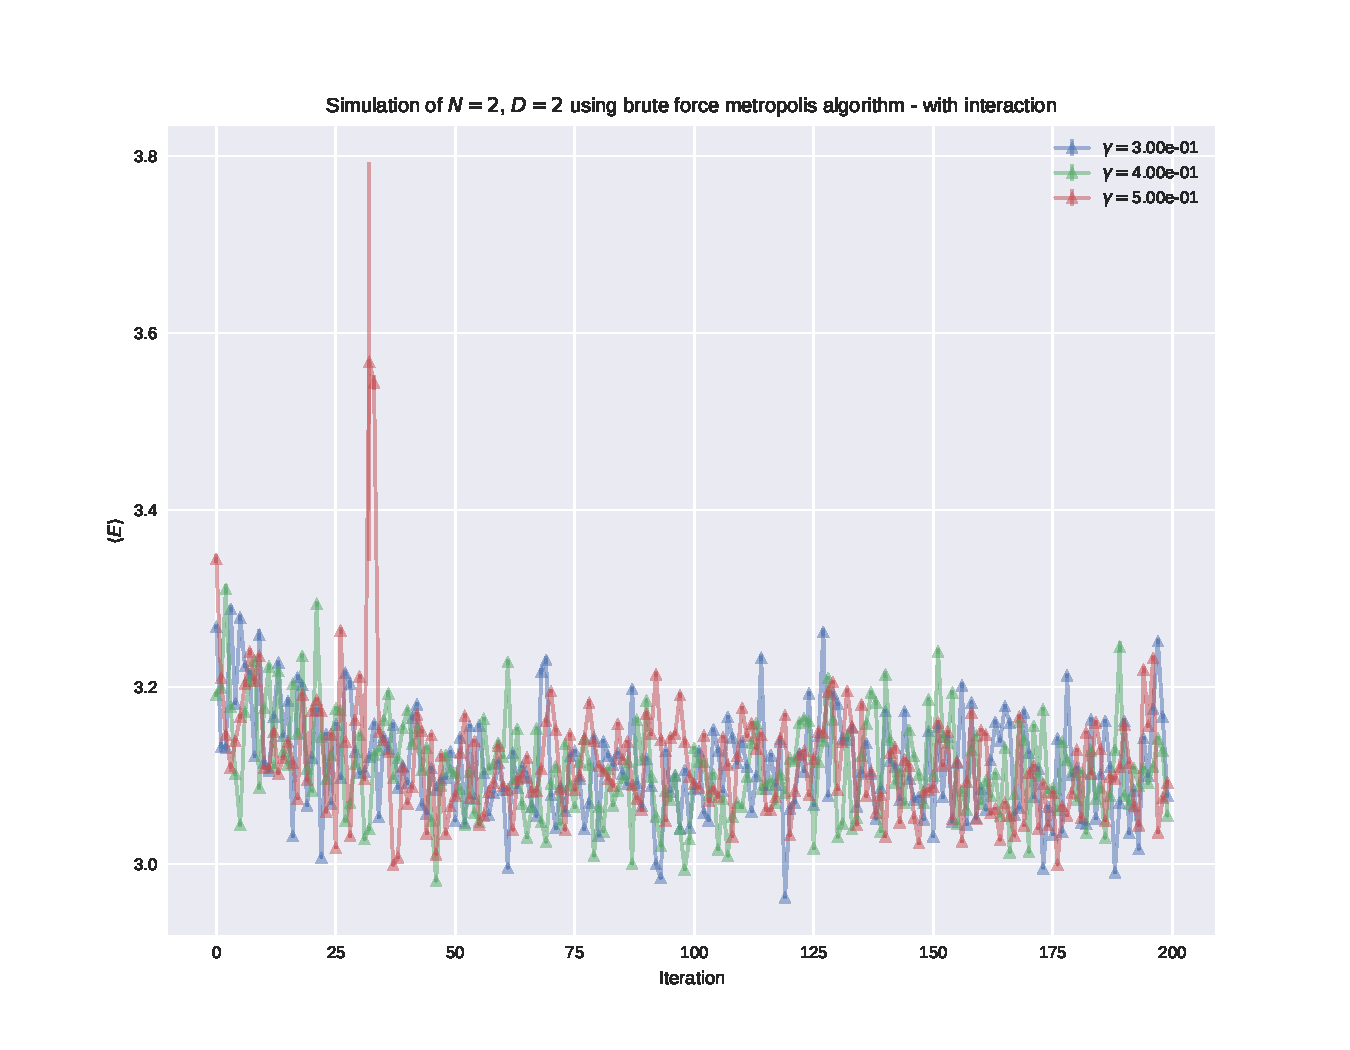
\includegraphics[width = \textwidth]{figures/interactive_naive.pdf}
\caption{Plotting the expectation value of the energy on the vertical axis versus the gradient descent step on the horizontal shows an oscillating behaviour. In this case the hamiltonian for the system has been modified to include a interactive term based on the distance between the two particles. As noted in the project description this system has an analytic minimum of 3 a.u. that the RBM touches, but does not stabilize to. See table \ref{tab:inter} for details on the stability for the different values of $\gamma$} \label{fig:inter}
\end{figure}
